Im 4. Kapitel dieser Arbeit sollen nun verschiedene Implementierungen und Ansätze erklärt und erläutert werden, Darauf sollen auf Herausforderungen eingegangen werden und ein kurzes Fazit zu den verschiedenen Ansätzen gezogen werden. Außerdem werden die wichtigsten Sachen der Implementierung hervorgehoben, um die Programmierung reproduzierbar zu machen, ohne Programmcode in diese Arbeit zu schreiben. Bei der Implementierung wird jeweils nur auf eine Android Implementierung eingegangen wie bereits in Kapitel 3 erklärt. 

\section{Entwicklung Nativer Android Applikation}
Die native Entwicklung ist die ursprünglichste von allen Arten. Android etwa wurde 2008 vorgestellt. 
Damals wurden die Apps für Android noch in Java entwickelt, eine Sprache die in der Anwendungsentwicklung damals und heute noch sehr gut bekannt ist und auch oft noch als Programmiersprachen an den Universitäten gelehrt wird. 
2019 jedoch änderte Google die offiziell bevorzugte Programmiersprache zu Kotlin. 
Kotlin ist von Jetbrains entwickelt um einen Ersatz für Java zu finden. 
Sie entwickelten eine Sprache die alle benötigten Funktionen für eine effektive Appentwicklung hat, jedoch genauso schnell kompiliert werden kann. 
Eine ähnliche Entwicklung fand auch bei Apple statt, die in Folge dessen von Objectiv-C zu Swift wechselten. 
Durch die Entwicklung eigener Sprachen haben sie die Kontrolle was in den Sprachen passiert und können diese perfekt für ihre Bedürfnisse anpassen.

Im folgenden wird die Implementierung eine native Android Applikation betrachtet werden.

\subsection{Grundlagen}

Die Entwicklung einer nativen Android \acp{App} besteht aus zwei separaten Teilen, Der erste Teil ist das Layout. Dabei wird ein Design für die Seite und eventuelle Elemente mit Hilfe der XML-Notation erstellt.
In der XML Datei wird ähnlich zu einer HTML Seite, die Oberfläche aufgebaut. Als Wurzelelement einer Seite ist ein Layoutelement. Neben einem linearem Layout oder einem Tabellenlayout, gibt es hier vor allem das so genannte \verb|Constraint-Layout|\footnote{https://developer.android.com/guide/topics/large-screens/support-different-screen-sizes}. 
Es ist das wichtigste Layout in Android, da wie der Name bereits andeutet, die Positionen der Elemente abhängig von anderen Elementen definiert ist. Durch diese Eigenschaft, eignet es sich besonders gut, um Designs für unterschiedliche Bildschirmgrößen zu erstellen. Es bietet dabei nicht nur die Möglichkeit, die Position, sondern auch die Größe abhängig davon zu definieren. Grundsätzlich hat Android nur zwei Optionen um die Größe eines Elements zu definieren. Es kann die größe des umgebenden Elements annehmen oder eine eindeutig definierte Größe. Durch das \verb|Constraint-Layout| kann jedoch über die Abhängigkeit zu beiden Seiten einer Richtung dazu gebracht werden, den verfügbaren Platz auszufüllen.

Der zweite Teil der Implementierung ist die Logik. Sie ist dabei in drei Klassen unterteilt. 
Die erste Klasse, die sogenannte Activity ist die Hauptklasse für eine Seite. In ihr wird alles gesteuert. Das Layout wird aufgerufen und der aktuellen Seite hinzugefügt, es werden alle Funktionalitäten zu den Elementen der Benutzeroberfläche hinzugefügt und ordnet der Oberfläche die Daten und den Listen ihre separaten Controller zu.

Dies ist ebenfalls die zweite Klasse. ListAdapter sind die Controller Klassen für Listen in Android. Listen werden dabei mit Elementen gebaut , die wiederverwendet werden, sobald sie außerhalb des Sichtfeldes sind. Dafür benötigt jede Liste einen Adapter, der dafür verantwortlich ist, die richtigen Elemente auszuwählen und Funktionalität und Daten hinzuzufügen.

Die dritte Klasse sind ViewModels\footnote{https://developer.android.com/topic/libraries/architecture/viewmodel}. Diese sind die Schnittstelle zwischen der Datenhaltung und der Activity. In einem ViewModel werden Daten abgefragt und Daten zwischengespeichert, die eine Konfigurationsänderung überstehen sollen. Diese sind etwa eine Änderung der Orientierung des Gerätes. Dies ist möglich, da ViewModels erst beendet werden, wenn ihre zugeordnete Aktivität final beendet wird. 
Durch die Nutzung kann die Performance verbessert werden. Es werden unnötige mehrfach Abfragen von Daten verhindert. Dazu kommt, dass ViewModels auf einem anderen Thread laufen als die Activity. Dadurch kann diese Events der \ac{UI} abfangen und weiterhin reagieren, während das ViewModel die nötige Daten sammelt.


\subsection{Genutzte Bibliotheken}
Die erste Bibliothek, die zur GraphQl-Kommunikation gewählt wurde, ist Apollo Kotlin. 
\TODO{Nochmal überlegen wegen dem wörtlichen Zitat}
"Apollo Kotlin ist ein GraphQL Client, der Kotlin und Java Modelle von GraphQL Queries erzeugt."\cite{Apollo_kotlin_docs} 
Anfänglich wird eine Konfigurationsdatei erstellt, in der Sachen wie der GraphQL-Endpunkt definiert werden. 
Danach stellt der Client eine Verbindung zu der GraphQL-\ac{API} her und fragt die Schnittstellendefinition ab, die im Anschluss gespeichert werden. 
Danach können die einzelnen GraphQL Befehle in einzelne Datein geschrieben werden. Aus diesen werden dann Modelle erstellt, die wie einfache Klassen im Applikationscode aufgerufen werden können.
Da Apollo die genaue Schnittstellendefinition hat, erzeugt es automatisch aus der \ac{JSON} Antwort des Servers ein Antwortobjekt und ordnet den einzelnen Stufen der Antwort die jeweiligen Datentypen zu.
Der Client wird der Applikation als globales Attribut hinzugefügt. Dadurch haben alle Activities darauf Zugriff und er kann einfach global geändert werden , wenn der Authentifizierungsstatus geändert wird.

Die zweite wichtige Bibliothek die genutzt wird, ist Room\footnote{https://developer.android.com/training/data-storage/room}. Sie ist Teil von Android Jetpack, dass ein Set an Bibliotheken ist, dass helfen soll, einfach und sauber Apps zu bauen, die über die verschiedenen Android-Versionen hinweg funktionieren \cite{Jetpack_android}. Room selber ist dabei der Teil, der es ermöglichen soll einen möglichst effizienten Datenbank Zugriff zu haben. 
Die Besonderheit ist, dass Room eine Zwischenebene darstellt, die sowohl die geschriebenen SQL Befehle überprüft und validiert, die asynchronität der Datenbankoperationen vereinfacht und durch Annotation redundanten Code verhindert \cite{Room_docs}.

Zum Speichern des Authentifizierungsstrings wurden sogenannte Shared-Preferences\footnote{https://developer.android.com/reference/android/content/SharedPreferences} genutzt. Sie sind ein weiterer Teil von Android Jetpack. Sie werden genutzt, um Key-Value Werte ohne großen Aufwand innerhalb der Applikation zu speichern. Sie können von innerhalb der ganzen Applikation abgefragt hinzugefügt, geändert oder gelöscht werden. Hierfür muss keine eigene Entität in der Datenbank angelegt werden und der Zugriff ist schneller. Sie sind jedoch nur für einfache Daten geeignet, da lediglich primitive Datentypen genutzt werden können. Daher werden sie vor allem für Werte wie Authentifizierung oder bestimmte Flags geeignet um den Status der App zu bestimmen.


\subsection{Fazit Android Nativ}
Nativ hat einige Vorteile. Es ist ein gut dokumentierter Ansatz, für den es für fast alle Probleme eine erprobte und funktionierende Lösung gibt. So war das Finden einer passenden GraphQL Bibliothek eine Leichtigkeit, da Apollo in diesem Bereich für Kotlin als Standardbibliothek gilt. Dazu kommt, dass es viele Bibliotheken gibt, die Google/JetBrains selber anbieten, um die Entwicklung von Apps zu vereinfachen und zu standardisieren.

Ein Vorteil der Layoutentwicklung in diesem Bereich ist, dass man das Layout in einer sofortigen Anzeige zusammenbauen kann und somit immer sofort sehen kann wie es aussieht. Jedoch ist dies eine Anzeige die nur die Oberfläche ohne Funktionalität oder von der Activity hinzugefügte Daten anzeigt. Wenn also hier Änderungen betrachtet oder getestet werden sollen, so muss die App neugebaut werden. Neben der Zeit, die es dauert die Änderungen zu laden, startet die App außerdem wieder vom Startbildschirm. Dadurch wird der Entwicklungsprozess verlangsamt und erschwert,


\section{Entwicklung einer hybriden Android Applikation mittels eines WebView-Containers}
Der zweite realisierte Ansatz ist eine hybride Applikation, die mit Kotlin implementiert wurde. 
Da einerseits die Implementierung der Web-Komponente durch viele verschiedene Ansätze umgesetzt werden kann und andererseits in diesem Fall bereits eine Webseite existiert, wird folglich nur auf die Implementierung der Schnittstelle eingegangen. 
Um ein besseres Verständnis über die Funktionalität des hybriden Ansatzes zu erhalten, wird auf die Nutzung eines Frameworks verzichtet und die Schnittstelle zwischen der eingebundenen Webseite und der Plattform nativ entwickelt.
Dabei wird die grundlegende Funktionalität ermöglicht. Eine umfänglichere Nutzung von Plattformfunktionalität wird in einem Exkurs vorgestellt.

\subsection{Grundlagen}
Um eine Minimalversion zu erhalten, wird eine native Applikation benötigt, die eine WebView-Komponente\footnote{https://developer.android.com/reference/android/webkit/WebView} enthält. Um die Funktionalität der Webseite zu ermöglichen, müssen unter Anderem die folgenden Aspekte beachtet werden.

So benutzen rund 98\% aller Webseiten JavaScript in ihrem Code, um zum Beispiel ein Menü ein oder auszublenden, ohne die Seite neu laden zu müssen \footnote{https://w3techs.com/technologies/details/cp-javascript}. 
Dazu muss jedoch JavaScript in der WebView aktiviert werden. 
Jedoch kann die Aktivierung von JavaScript ein Sicherheitsrisiko darstellen. So können etwa fremde Webseiten ebenfalls versuchen, auf das Gerät zuzugreifen \cite{webview_javascript_security}. 
Daher sollte die Implementierung externe Links erkennen und diese in einem externen Browser-Fenster öffnen.
Die Links können dabei entweder in dem normalen Browser des Gerätes geöffnet werden oder in einem CustomTabsIntent\footnote{https://developer.android.com/reference/androidx/browser/customtabs/CustomTabsIntent}.
Dadurch entsteht ein Browsertab in der eigenen Applikation, dass etwa in der Akzentfarbe der Applikation angepasst werden kann um eine Zugehörigkeit erkennbar zu machen, jedoch dennoch einen externen Browser zu erhalten. Es ist jedoch durch die angezeigte Funktionsleiste mit angezeigter URL am oberen Bildschirmrand dennoch als externer Inhalt erkennbar.

Um dies zu ermöglichen muss jedoch die aufgerufene URL abgefangen werden und entschieden werden, wie mit der aufgerufenen URL verfahren werden soll. So ist eine einfache Grundkonfiguration, dass alle URLs die zur angezeigten Webapplikation gehören zugelassen werden, während externe Links weitergeleitet werden.

Eine letzte Konfiguration, die benötigt wird um etwa das Login mit Google zu ermöglichen ist das Setzen eines UserAgentStrings. Er ist eine Text Flagge, die in einem HTTP-Paket zu finden ist. Sie beinhaltet Informationen zu dem benutzten Client oder der genutzten Hardware. Außerdem wird sie auch genutzt, um verdächtige Pakete heraus zu filtern\cite{UserAgentString}. So filtert Google LogIn-Anfragen herraus, bei denen der UserAgent nicht gesetzt ist. Dieser kann durch das Setzen der Variable auf dem Webcontainer definiert werden.

Mit diesen Konfigurationen ist eine grundsätzliche Funktionalität einer Webapplikation sichergestellt. So kann an diesem Punkt theoretisch eine erste Version veröffentlicht werden. Jedoch ist an diesem Punkt dem Nutzer immer noch sichtbar, dass es sich bei dem Inhalt um eine Webseite handelt. Um dies zu verhindern können über die Layoutdatei native Elemente über oder um das WebView anlegen. So kann etwa ein Home Button dem Layout hinzugefügt werden, um der Anzeige native Elemente hinzuzufügen.

Neben der Konfiguration des Aussehens kann die WebApplikation noch in der benutzung von Gerätefunktionalität angepasst werden. Auf eine derartige mögliche Erweiterung soll deswegen im Folgenden Exkurs etwas eingegangen werden.

\subsection{Exkurs: Nutzung von Plattformfunktionalität}
Wie in Kapitel \ref{cha:3_hybrid} erwähnt, haben hybride Applikationen die Möglichkeit auf Plattformfunktionalität zuzugreifen. Dies ist der Teil, den Frameworks typischer Weise bereits umgesetzt haben und um die ein Entwickler sich normalerweise keine Gedanken machen muss. Jedoch wird in dieser Arbeit kein Framework genutzt, um einen Möglichen Ansatz zu zeigen, dies in die eigene Applikation zu integrieren. So kann ein von der App initialisiertes und der WebView hinzugefügtes WebAppInterface\footnote{https://developer.android.com/guide/webapps/webview\#BindingJavaScript} direkt aus dem JavaScript der Webseite aufgerufen werden \cite{webview_javascript_security}. Dafür werden Objekte und ihre öffentlichen Methoden dem Webcontainer unter einem definierten Namen zur Verfügung gestellt. Es können dabei sowohl Daten gesendet als auch empfangen werden.

Auch kann aus der Applikation JavaScript Code aufgerufen beziehungsweise ausgeführt werden. Dafür wird mit der loadUrl Methode, die in der WebView normalerweise einen Link aufruft, JavaScript-Code mit dem Präfix \verb|"javascript:"| der WebAnwendung hinzugefügt \cite{webview_javascript_security}. Dies kann sowohl selbst geschriebener Code als auch ein Aufruf bereits definierter Methoden sein. Dies zeigt jedoch, dass auch innerhalb der Webanwendung ein besonderes Augenmerk auf die Sicherheit gesetzt werden muss, da unter Umständen neben der Applikation, auch die Webseite angreifbar ist. So könnten bösartige Applikationen versuchen, über die JavaScript Schnittstelle eigenes JavaScript auszuführen, um so etwa den aufgerufenen Webserver zu attackieren. Dies ist möglich, da JavaScript-Code, der über loadUrl hinzugefügt wurde, im aktuell angezeigten Kontext gleichwertig wie von von der Webanwendung stammendes JavaScript ausgeführt wird \cite{webview_javascript_security},

\subsection{Fazit hybride Implementierung}
Ein Vorteil dieser Implementierung ist die Entwicklungsgeschwindigkeit, die erreicht werden kann, wenn bereits eine Webanwendung existiert. Anstatt die Anwendung komplett neu zu schreiben und somit multiple Implementierungen der Anwendungslogik zu erstellen, kann mit diesem Ansatz die Webanwendung in eine native Applikation eingebettet werden.
Ein weiterer Vorteil ist, dass durch die Nutzung der extern gehosteten Webanwendungen, Änderungen am Inhalt der angezeigten Anwendung nicht erst auf den Geräten der Nutzer installiert werden müssen, sondern direkt nach einem Neuladen der Webseite bei allen Nutzern verfügbar ist. 
Dazu kommt, dass an der eigentlichen Applikation nur sehr selten Änderungen durchgeführt werden müssen, da hier in den meisten Fällen nicht viel Logik verbaut ist.

Ein Nachteil ist, dass in diesem Fall die App nur nutzbar ist, wenn eine aktive Internetverbindung besteht, da der Großteil der angezeigten App, aus der Webseite bestehen. Dazu kommt, dass der Programmier- und Wartungsaufwand steigt, wenn eine umfangreiche Nutzung von Gerätefunktionalität geplant ist. Des Weiteren wird bei dieser Implementierungsart wieder eine eigene Implementierung des nativen Containers für jede Plattform benötigt., dies kann jedoch durch die Nutzung eines Frameworks verhindert werden. Ein Problem für diese Art der Entwicklung sind jedoch die Review Guidelines des Apple AppStores\footnote{https://developer.apple.com/app-store/review/guidelines/\#minimum-functionality}. Diese legen fest, dass die App nicht einfach nur ein Container für eine Webseite sein darf, sondern zu großen Teilen aus für den Nutzer nützlichen Funktionalitäten bestehen muss. Dadurch ist es wahrscheinlich, dass eine Implementierung im Umfang der hier dargestellten Applikation von Apple nicht veröffentlicht werden würde, wenn nicht noch zusätzliche Funktionalität hinzufügt wird.

Einige der Vor und Nachteile sind jedoch stark von der hier vorgestellten Implementierung abhängig. So wird etwa durch die Nutzung einer lokal gespeicherten Implementierung eine offline Funktionalität erreicht, jedoch müssen dadurch Änderungen über den normalen Updateprozess der einzelnen Plattformen verteilt werden.
Auch kann die gesamte Implementierung durch die Nutzung von Frameworks erledigt werden, jedoch muss die Webseite dann an dieses Framework angepasst werden und die nutzbare Funktionalität durch die implementierten Lösungen eingeschränkt sein. 


\section{Entwicklung Cross-Plattform Applikation mit Flutter}
Der dritte Ansatz der hier erklärt werden soll, ist eine Cross-Plattform-Implementierung mit Hilfe des Flutter Frameworks.

\subsection{Flutter Grundlagen}
Flutter ist ein 2017 von Google veröffentlichtes Framework das mittlerweile zum bedeutendsten Cross-Plattform-Framework geworden ist\cite{statist_CP_Framework}. Neben viel Aufmerksamkeit von Entwicklern haben auch Firmen großes Interesse an Flutter. So hat etwa die Firma hinter Ubuntu, Canonical, angekündigt, dass alle von ihnen entwickelten Anwendungen, in Flutter programmiert werden\cite{Ubuntu_Flutter}. Als Programmiersprache wird dabei Dart benutzt, die je nach Plattform, mit unterschiedlichen Compilern übersetzt wird,

Eine Grundlage von Flutter ist \verb|Composition over inheritance|. Dieses Konzept ist besonders gut sichtbar beim Aufbau der Nutzeroberfläche. Alles ist ein Widget. Bis auf die Geschäftslogik ist alles, wie etwa Gestenerkennung, Layouthelfer und tatsächlich Angezeigte Elemente ein Widget\cite{Thiele_2018}. Dabei werden Widgets baumartig verschachtelt, wobei die meisten Widgets wieder ein oder mehrere Kinderelemente haben, die ein Widget sind. In Abbildung \ref{fig:flutter_layout_tree} etwa ist der Widget-Baum einer Menüleiste zu sehen. Dabei sind Container Elemente, die um Widgets gebaut werden, um weitere Sachen wie Abstände oder anderes hinzufügen. Nur bei Widgets wie in diesem Fall etwa Text oder Icon, stoppt der Baum, da diese keine weiteren Kinder haben.

\begin{figure}[ht]
  \centering
  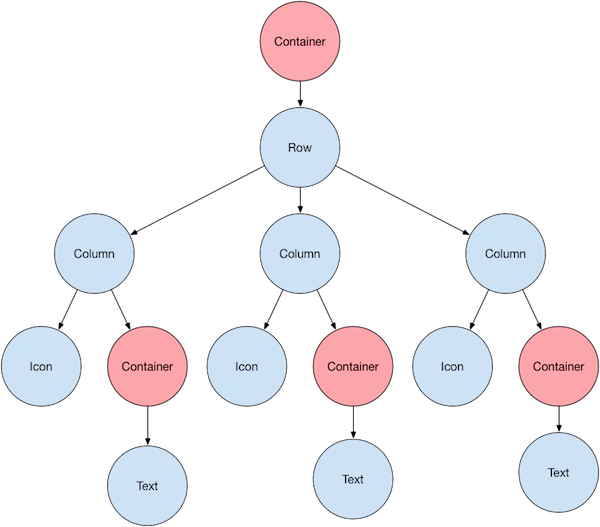
\includegraphics[height=7cm,keepaspectratio]{images/sample-flutter-layout.png} 
  \caption{Hierachie einer Menüleiste Quelle\protect\footnotemark}
  \label{fig:flutter_layout_tree}
\end{figure}

\footnotetext{https://docs.flutter.dev/development/ui/layout}

Anders als bei der nativen Implementierung wird in Flutter das Layoutfile mit der Funktionalität dahinter gemischt. Das bedeutet, dass die Funktionalität direkt beim definieren eines Knopfes zugeordnet wird. Dafür muss lediglich das Widget in den Baum eingefügt werden und danach das entsprechende Attribut gesetzt werden. Dadurch ist alles an einem Ort.

Da Flutter einen großen wert auf Perfomance legt, ist eine Änderung auf der \ac{UI} so gebaut, dass nur Elemente neu gebaut werden, die ihren Inhalt geändert haben. Dafür hat Flutter für \verb|Stateful Widgets|, die eine extra State Klasse besitzen. In diesem werden Daten gespeichert und sobald er sich ändert, registriert Flutter die Änderung und baut daraufhin das geänderte Widget und die in der Hierachie folgenden neu\cite{9623025}. Dadurch kann häufiges und vor allem vollständiges Neubauen des Widgetsbaums verhindert werden. Jedoch benötigt nicht jedes Element einen State. Wenn etwa bereits zum Zeitpunkt des Erzeugens des Widgets, alle Daten feststehen und auch nicht mehr geändert werden, dann wird kein State benötigt und es reicht ein \verb|Stateless Widget| für die Implementierung\cite[Kapitel~4]{Flutter_Recipes}. Dadurch wird einerseits die Implementierung eines States ersparrt und bei einem Neubau des Baums, kann das Widget-Element wieder genutzt werden und muss lediglich neu gerendert werden, was bei Flutter jedoch sehr performant ist.

Um sich wiederholenden Code zu sparen, kann in Flutter einfach ein eigene Widget geschrieben werden, dass im gesamten Projekt wie jedes andere Element auch, in den Widget-Tree eingefügt werden kann. Das Erstellen eines Widgets ist dabei der selbe Prozess wie das erstellen einer Seite. Es wird ein Knoten Element gewählt und dann mit anderen Elementen kombiniert, um die gewünschte Oberfläche zu erhalten. Außerdem muss entschieden werden, ob es ein Stateful oder Stateless Widget ist. Je nachdem muss noch ein zusätzlicher State implementiert werden.


\subsection{benutzte Plugins}
Das erste Plugin dass zu erwähnen ist, ist \verb|graphql\_flutter|\footnote{https://pub.dev/packages/graphql\_flutter}. Es ist ein Packet, dass ähnlich zu dem bereits erwähnten Apollo GraphQL einen Client zur Kommunikation mit einer GraphQL Schnittstelle. Damit der Client in allen Pages und Widgets verfügbar ist, muss die Konfiguration als Wurzel der Applikation gesetzt werden. Danach kann entweder über ein Widget oder über eine programmierte Funktion Die verschiedenen GraphQL Funktionen ausgeführt werden. Es ist ein Open Source von einer Community geschriebenes Plugin. Dies ist auch in der Nutzung spürbar. So sind einige Funktionalitäten nicht so sehr ausgereift wie bei der Apollo Implementierung. So muss etwa auf die einzelnen Felder der Antwort mit der JSON Zugriff \verb|Antwort.data[\"Feldname\"]|. Die Gefahr ist dabei hoch, dass durch ein Tippfehler der Zugriff schief läuft. Durch die Entwicklung von einer Community ist es allerdings einfacher Hilfe zu bekommen. So wurde während der Entwicklung ein paar Fragen auf dem dafür eingerichteten Discord-Server eingestellt, die professionell innerhalb einiger Stunden beantwortet wurden.

Das zweite wichtige Plugin ist Hive\footnote{https://pub.dev/packages/hive}. Es ist ein einfacher und schneller Key-Value Speicher, der Daten auhc über einen Neustart der App hinaus, in einer Datei innerhalb des Applikationsordner speichert. Er wird dafür genutzt, um den Identifikationsstring für den Server zu speichern. Es ist vergleichbar mit den \verb|SharedPreferences| der nativen Entwicklung vergleichbar, ist jedoch umfangreicher, da auch Objekte mit der richtigen Konfiguration gespeichert werden können und ist beim lesen vergleichbar beziehungsweise beim Schreiben schneller.

Ein drittes Plugin das hier noch erwähnt werden sollte ist \verb|simple\_gradient\_text|. Es ist ein Paket um ein Text mit Farbverlauf in der Schrift zu haben. Es ist also lediglich ein Paket, das zur Erstellung der Oberfläche genutzt wurde und ist dementsprechend hier nicht so wichtig. Jedoch zeigt sich hier wieder der Vorteil an einer aktiven Community. Bei der Installieren des Paketes gab es anfänglich einige Probleme, da es auf Android funktionierte aber auf anderen Plattformen nicht. Nach einer Unterhaltung mit dem Entwickler über ein erstelltes Problem auf GitHub ergab sich, dass das Plugin eine höhere Minimalversion von Dart benötigte, als in meiner Konfiguration eingestellt. Dadurch konnte bei mir der Fehler einfach behoben werden. Daraufhin wurde die Dokumentation des Paketes sowohl auf GitHub und dem zentralen Plugin Verzeichnis aktualisiert und um die entdeckte Anforderung erweitert.

Als letzte wichtige Bibliothek, wurde \verb|sqflite\_common\_ffi|\footnote{https://pub.dev/packages/sqflite\_common\_ffi} für die Implementierung der Datenbank genutzt. Es ist eine Bibliothek, dass auf Basis von \verb|sqlite3| eine Datenbankimplementierung für alle Plattformen anbietet.
Diese wird beim Start der Anwendung geöffnet und ist danach in der kompletten Anwendung verfügbar.
Mit ihre können alle gängigen \ac{CRUD}-Operationen durchgeführt werden. Die Implementierung ist dabei denkbar einfach.
Zum erstellen der Tabelle muss lediglich der SQL Befehl zum erstellen ausgeführt werden und danach kann über dedizierte \verb|insert| und \verb|query| Methoden die Daten gespeichert beziehungsweise abgefragt werden.
Nebenbei kann jede Art von SQL-Befehl ausgeführt werden, um Befehle auszuführen, die über die normale Implementierung hinaus gehen.


\subsection{Exkurs: Platform spezifische Funktionalität entwickeln}
Im Verlaufe der Entwicklung kann es vorkommen, dass eine gewisse Funktionalität, die essentiell für die Anwendung ist, bisher nicht implementiert wurde oder die Verfügbaren Bibliotheken nicht die gewünschte Funktionalität hat oder gewisse Plattformen nicht unterstützt werden. Für diesen Fall kann eigener Plattformcode geschrieben werden. Dafür wird einerseits der benötigte Dart Code geschrieben und dann der jeweilig notwendige Plattformcode. Zur Kommunikation zwischen den Verschiedenen Teilen werden dabei Plattform-Channels genutzt.\cite[Kapitel~12.3]{Flutter_Recipes}

Durch die Nutzung eines Kanals zur Kommunikation erlaubt es die Ausführung des Plattform Codes auf einem separaten Thread. Dadurch kann dieser asynchron ausgeführt werden und eine Blockade des Threads auf dem die \ac{UI} ausgeführt wird, verhindert werden\cite{plattform_code_flutter}.

Um weiteren Entwicklern die entwickelte Erweiterung zur Verfügung zu stellen kann außerdem das Plugin in das offizielle Repository von Flutter hochladen.

Es ist also möglich benötigte Funktionalität hinzuzufügen, solange sie auf den einzelnen Plattformen möglich ist. Jedoch werden für eine derartige Entwicklung das nötige Wissen benötigt, um den Plattformcode zu schreiben.

\subsection{Exkurs: Firebase}
Ein weiterer Aspekt, warum Flutter gerade bei kleineren App-Projekten gern genutzt wird, ist die umfangreiche Integrationsmöglichkeit von Firebase. Eine aktuelle Untersuchung ergab, dass in Android Applikationen die eine Analyse Software integriert haben, 92\% der weltweiten Applikationen, Firebase nutzt \cite{statist_analytics_SDK}.

Firebase ist eine Backend-as-a-service Lösung, die dabei helfen soll, schnell und einfach Anwendungen zu entwickeln und zu betreiben\footnote{https://firebase.google.com/}. Es ist also eine Sammlung von verschiedensten Tools und Plugins, die einem Entwickler die Möglichkeit geben soll, sich auf Design und Funktionalität der App konzentrieren zu können. Es umfasst Tools wie eben Analyse Software um Nutzungsdaten zu sammeln und zu analysieren, ein fertiges Chatsystem oder auch eine Cloud gestützte Datenbank Lösung. So schreiben Guzzi et Al, dass entweder ein Team an Entwickler angestellt werden müssten, das in monatelanger Arbeit ein Backend System programmieren würde, um dann eine Schnittstelle zu einem Backend zu bauen. Andererseits kann auch ein bereits bestehendes System gennommen werden. Mit Firebase werden tausende Zeilen Code eingespart und erhält dabei die Möglichkeit, asynchrone Aufrufe und nebenläufige Prozesse für eine reaktive App zu nutzen \cite[p.~608]{Flutter_Apprentice}.

Um eine Datenbank für seine App zu erstellen sind es wenige Schritte. So kann auf der Webseite von Firebase eine neue Datenbank angelegt werden. Danach wird die erzeugte Konfigurationsdateien für die jeweiligen Plattformen heruntergeladen. Diese werden den jeweiligen Implementierungen hinzugefügt. Danach müssen die Datenstrukturen lokal in der App entworfen werden und eine Verbindung hergestellt. Dafür werden die Daten-klasse mit JSON Konvertierungen, ein \ac{DAO} mit einer Methode zum speichern und holen der Daten und zuletzt noch einen Provider erzeugt. Außerdem besteht die Möglichkeit, neben einer online Datenbank ebenfalls eine offline Version hinzuzufügen, die synchronisiert wird, sobald eine Internetverbindung hergestellt wird \cite{Flutter_Apprentice}.

Ein weiterer Pluspunkt ist die Integration von Firebase-Authentifizierung. Es bietet eine fertige Lösung zur Authentifizierung von Nutzern. Es besteht außerdem die Möglichkeit, Benutzer zu kategorisieren beziehungsweise die Nutzung einzuschränken. So kann über Regeln in der Firebase-Website, präzise definiert werden, welcher Nutzer auf welche Daten zugreifen kann. Weiter können Nutzer auch von der Nutzung des Dienstes ausgeschlossen werden oder nur bestimmte Emailadressen zugelassen. Es bietet also ein vielseitig und umfangreiches Nutzerverwaltungstool \cite{Flutter_Apprentice}.

Firebase ist natürlich nicht nur für Flutter verfügbar, sondern genauso für die verschiedensten Programmiersprachen der Plattformen Android, iOS oder auch Web. Dennoch ist Flutter und Firebase ein interessantes Gesamtsystem. Denn durch Flutter muss lediglich einmal der Code zum Zugriff auf die Datenbak oder die anderen Dienste geschrieben werden. So wird nicht nur weiter Entwicklungszeit um sehr ähnlichen Code zu schreiben, sondern verhindert gleichzeitig eine unterschiedliche Definition der Entitäten oder anderen Elementen. Außerdem ist dadurch ein problemloser Wechsel von einem System zu einem anderen Möglich, da alle Anwendungen auf egal welcher Plattform gleich sind.

\subsection{Conclusion Flutter}
Durch die hier beschriebene Entwicklung kann mit Hilfe von einem Code, eine Anwendung geschrieben werden, die sowohl auf Android, iOS, Windows, Mac und Linux läuft. Lediglich die Web Implementierung funktioniert nicht, da der GraphQL Client hier keine richtige Verbindung erstellen kann. Für alle anderen Plattformen muss lediglich die Unterstützung deklariert, der Code in Plattform spezifischen Code compiliert und am Ende ausgeführt werden.

Das Tempo mit dem eine Flutter Anwendung entwickelt werden kann ist ähnlich wie eine einzelne native Implementierung. Dabei entsteht aber, wie bereits erwähnt, nicht nur die Implementierung für eine Plattform, sondern 5. Selbst wenn der Fokus der Entwicklung zuerst nur auf einer Plattform liegt, kann es sinnvoll sein Flutter zu nutzen um in Zukunft weitere Plattformen hinzuzufügen. Denn alle Plattformen können nachträglich noch exportiert werden.

Jedoch ist dies natürlich nicht immer möglich. Denn etwa der GraphQL Client ist nicht mit einer Web-Version kompatibel. Daher sollte bei der Wahl der Pakete darauf geachtet werden, welche Packete ausgewählt werden, um eine Inkompatibilität mit den gewünschten Plattformen zu verhindern. Wie bereits ausgeführt, kann versucht werden, solche Probleme durch eine eigene Implementierung zu lösen, dies ist jedoch mit einem erhöhten Aufwand und nötigen Wissen verbunden. Dabei ist die eigentliche Implementierung an sich nicht das eigentliche Problem, da auch hier dann native externe Bibliotheken genutzt werden können, jedoch ist die Konfiguration der Kommunikationsschnittstellen mitunter recht kompliziert und müssen sinnvoll implementiert sein, um die Performance nicht erheblich zu schwächen.

Flutter ist außerdem noch recht neu. So werden bei regelmäßigen Updates auch Änderungen eingeführt, die die Qualität und Entwicklung verbessern, jedoch dabei auch umfangreiche Änderungen in allen Applikationen notwendig macht. So wurde etwa ein Update veröffentlicht, dass das Nullsafety verbessern sollte. In Folge dessen musste jede Bibliothek angepasst und auch große Teile von Applikationen angepasst werden. Dadurch sind auch einige Anleitungen für Flutter veraltet und funktionieren in der aktuellsten Version nicht ohne Anpassungen.

Ein letzter Punkt ist, dass es keine Liste der verfügbaren Widgets innerhalb der Entwicklungsumgebung gibt. So muss alles, was nicht bereits bekannt ist gegoogelt werden. Hier wäre eine Übersicht über die typischen Elemente hilfreich um gerade für Anfänger den Einstieg zu erleichtern.

\section{Entwicklung einer gemischten Applikation mit WebView und Flutter}
Die vierte Implementierung ist dem gemischten Ansatz zuzuordnen. Sie besteht aus der Kombination einer hybriden Applikation und einer cross-kompilierten Applikation.
Hierbei sind die einzelnen Ansichten entweder eine mit Flutter implementierte Seite oder eine mittels WebView integrierte Ansicht der Webseite.
Durch diese Kombination soll die bereits bestehende Webseite wiederverwendet werden, während gleichzeitig bestimmte Teile des Systems für die mobile Nutzung angepasst werden und durch eigens programmierter Flutter Seiten ersetzt werden.
Dadurch kann ein Teil der Neuimplementierung vermieden werden, während die Nutzererfahrung für die neuen Plattformen optimiert werden kann.
Dabei soll weiterhin die Möglichkeit bestehen, die individuellen Applikationen aus einer gemeinsamen Code-Basis zu kompilieren.

\subsection{Grundlagen}
Da es sich wiederum um eine Flutter Applikation handelt gelten die selben Grundlagen wie in Kapitel \ref{cha:4_3_1}.
Zusätzlich wird nun eine WebView-Komponente hinzugefügt und zwischen Web-Oberflächen und Flutter-Seiten hin und her gewechselt.
Da dies kein weit verbreiteter Ansatz ist und es folglich keine offizielle Dokumentation oder Anleitungen für diesen Ansatz gibt, mussten hierzu einige Herausforderungen überwunden werden, die im Folgenden erläutert werden sollen.

Die Integration der Webseite ist ähnlich zum Vorgehen bei der hybriden Applikation. So werden aufgerufenen URLs abgefangen und es wird sich für eine von drei Vorgehensweisen entschieden. So werden Links zu externen Webseiten im Browser des Gerätes geöffnet. URL´s der eigenen Web-Anwendung, bei der die Web-Ansicht genutzt werden sollen, werden in der WebView geladen. Letztlich werden URL's, die zu Seiten gehören, die durch eine Flutter Seite angezeigt werden sollen, verworfen und die entsprechende Flutter Seite mit eventuell vorhandenen Parametern aus der URL geladen. 
Dementsprechend muss die Analyse und darauf folgende Unterscheidung der URLs deutlich feingradiger stattfinden.

Flutter beendet standardmäßig alle nicht mehr angezeigten Seiten und löscht dabei auch mögliche gespeicherte Informationen. So etwa auch die Navigationshistorie der WebView.
Da diese allerdings benötigt wird, um innerhalb der Webanwendung zurück zur vorherigen Seite zu navigieren, wird folglich eine Möglichkeit benötigt, um die Daten der WebView zu speichern. Dafür wurde das von Flutter bereitgestellte \verb|AutomaticKeepAliveMixin|\footnote{\url{https://api.flutter.dev/flutter/widgets/AutomaticKeepAliveClientMixin-mixin.html}} verwendet. 
Wie der Name beschreibt, werden damit die States von Widgets markiert, um zu bewirken, dass die Garbage Collection diesen nicht löscht. 
Bei einem erneuten Aufruf der Seite wird dann der noch vorhandene State geladen. Dadurch wird ein Zurücknavigieren in der Webseite auch nach dem vorherigen Verlassen der Web-Ansicht weiterhin möglich.

Es existiert außerdem bei diesem Ansatz eine zusätzliche Herausforderung bei der Navigation.
Dabei ist das Navigieren zu einer neuen Seite ohne Probleme durch die Navigation der WebView möglich. Die aufgerufene URLs werden abgefangen und ,wie bereits erklärt, weiterverarbeitet. Aus einer Flutter-Ansicht heraus wird dann entweder zu einer anderen Flutter-Ansicht navigiert oder die neue URL in der WebView aufgerufen. Bei der Rückwärtsnavigation ergibt sich jedoch folgendes Problem. Zwar kann die Flutter Navigation ohne Probleme von einer Flutter-Seite in die WebView zurückkehren, wo dann die Navigation der WebView übernimmt. Wurde jedoch in vorherigen Verlauf zu einer Flutter Webseite navigiert, so ist diese im Verlauf der Webseite enthalten. Da die Methode, welche über das weitere Verfahren der URL entscheidet, lediglich bei vorwärts navigieren aufgerufen wird, würde fälschlicher Weise die Webseite angezeigt werden und nicht die angepasste Flutter-Seite.
Um diese Herausforderung zu überwinden, wurden zwei mögliche Lösungen erarbeitet:
\begin{enumerate}
    \item Eine eigene Navigation programieren, in der genau definiert werden kann, wann eine URL als Webseite geladen wird und wann eine Flutter Seite aufgerufen wird. 
    \item Jedes mal, wenn von einer Flutter Seite zurück in eine WebView gewechselt wird, eine neue WebView erzeugen und somit den bereits vorhandenen Entscheidungsprozess für URLs nutzen. 
\end{enumerate}

Beide Lösungen haben Vor und Nachteile. So benötigt der erste Ansatz weniger Ressourcen, da lediglich eine WebView genutzt werden kann. Jedoch wird hier ein hoher Implementierungsaufwand benötigt, um eine angepasste Navigation zu schreiben. 
Beim zweiten Ansatz ist die Performance zwar schlechter, jedoch kann die von Flutter bereitgestellte Navigation genutzt werden. Somit können Fehler bei der Implementierung und ein zusätzlicher Programmieraufwand vermindert oder vermieden werden.
Wenn zusätzlich sinnvolle Punkte in der App definiert werden, an welchen die Navigationshistorie der Flutter-Navigation gelöscht wird, können folglich alte WebView Konfigurationen von der Garbage Collection gelöscht werden und folglich die vom Ansatz benötigten Ressourcen reduziert werden. Daher wurde für die Implementierung die zweite Lösung gewählt. 

Eine letzte Herausforderung war die Kombination der verschiedenen Technologien. Beispielsweise wurde bei der Web-Implementierung eine sogenannte Live-Komponente benutzt. Diese sorgt dafür, dass bei einem Wechsel von einer Seite zu einer anderen, keine neue URL geladen wird, sondern lediglich der Inhalt dynamisch nachgeladen wird. Dies lag zum Beispiel bei der Umsetzung des Chats vor. So war die Überssichtsseite der Konversationen mit der Anzeige der einzelnen Chats über diese Technologie verbunden. Deshalb konnte nicht ,wie ursprünglich geplant, lediglich die Chat-Seite durch Flutter ersetzt werden, sondern es musste auch die davorliegende Übersichtsseite umgesetzt werden.

\subsection{Benutzte Packages}
Es wurden die selben Erweiterungen wie in der Flutter Implementierung benutzt. Zusätzlich wurde ein WebView-Package benötigt, um die hybride Implementierung zu ermöglichen. Hierfür wird das von Flutter veröffentliche \verb|webview_flutter|\footnote{\url{https://pub.dev/packages/webview\_flutter}} Package genutzt. Anzumerken ist, dass die Wahl der richtigen Erweiterung kompliziert war, da keine der Optionen alle Plattformen unterstützte. Letztendlich wurde die offizielle Erweiterung gewählt, welche lediglich Android und iOS unterstützt.

\subsection{Fazit gemischte Implementierung}
Im Vergleich zur hybriden Implementierung ist mehr Implementierungsaufwand nötig, da Teile der Webseite durch eine eigene Implementierung ersetzt werden. Jedoch konnte die Benutzbarkeit der Applikation verbessert werden, da durch das gezielte Ersetzen der Webanwendung eine für die Plattform speziell angepasste Funktionalität oder Aussehen erreicht werden kann. Dabei kann Implementierungszeit im Vergleich zur nativen beziehungsweise cross-kompilierten Applikation gespart werden, wenn die Teile der Webanwendung, die von einem derartigen Umbau nicht profitieren, weiterhin als Webseite angezeigt werden.
Außerdem ermöglicht dieser Ansatz, dass ein Umbau von Webanwendung zu Applikation iterativ möglich ist und somit eine erste Version früher veröffentlicht werden kann.

Jedoch entstanden durch die Nutzung des gemischten Ansatzes einige Herausforderungen, für die es wenig Hilfestellungen in Foren oder Dokumentationen gibt. Daher ist dieser Ansatz mit einem erhöhten Aufwand verbunden und es besteht die Gefahr, dass etwa eine reine cross-kompilierte Implementierung schneller entwickelt werden könnte.